% Chapter 1

\chapter{Business Process Mining} % Main chapter title

\label{Chapter2} % For referencing the chapter elsewhere, use \ref{Chapter1} 

%----------------------------------------------------------------------------------------

% Define some commands to keep the formatting separated from the content 
%\newcommand{\keyword}[1]{\textbf{#1}}
%\newcommand{\tabhead}[1]{\textbf{#1}}
%\newcommand{\code}[1]{\texttt{#1}}
%\newcommand{\file}[1]{\texttt{\bfseries#1}}
%\newcommand{\option}[1]{\texttt{\itshape#1}}

%----------------------------------------------------------------------------------------

\section{Basic Concepts of Process Mining}
Before introducing the Data-aware Heuristic Miner, the basic concepts of Process Mining will be introduced in order to provide a good understanding of Business Process Mining beforehand.\\
\noindent The work in the field of Processes can be seen as a process it self. In order to distinguish the focus of this seminar paper from other fields of research, the main steps are displayed in the following figure.

\begin{figure}[H]
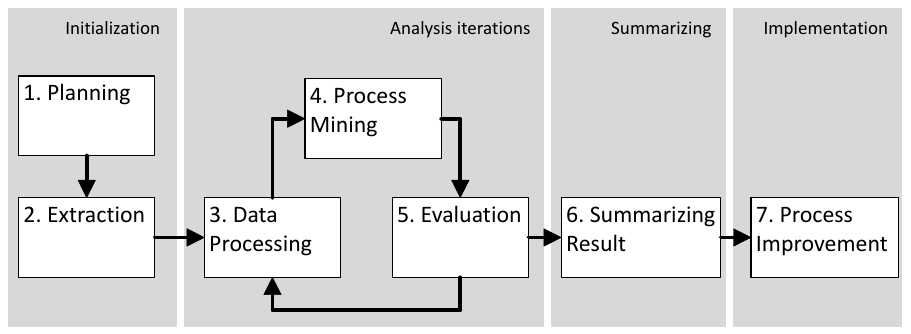
\includegraphics[width=14cm]{Chapters/Notizen_Graphics/ProcessMiningSteps.jpg}
\caption{Steps in Process Mining\protect\cite{Buijs2017}} 
\end{figure}

\noindent The DHM is a new mining method and thus the main focus lies on step 4. and only partly on 3. and 5. when reproducing the results and testing further functionalities in ProM. \protect\cite{Buijs2017}\\


\subsection{Event logs, Petri nets and model criteria}
Event logs store information about \textbf{activities} and each execution of a process produces a sequence of \textbf{events}. Events are stored with attributes $A$ and values $U$ in traces $\sigma \in \mathscr{L}$.\\
Thus an event log $L = (E, \Sigma, \#, L)$ consists of:


\begin{itemize}
\setlength{\itemsep}{3pt}
\item{$E$ - a finite set of unique event identifiers}
\item{$\Sigma \subseteq U$ - a finite set of activities}
\item{$\# : E \rightarrow (A \nrightarrow U)$ - attribute values recorded for an event}
\item{$\mathscr{L} \subseteq E\text{*}$ - the set of traces over E}
\item{$\sigma \in \mathscr{L}$ - traces, which record the sequence of events for
one process instance - each event occurs only in a single trace}
\end{itemize}

\noindent In the following figure this can be seen for three traces with attributes \textbf{act}ivity, \textbf{p}riority, \textbf{n}urse and \textbf{t}ype. The Hospital Billing Example will be used through this paper for a better explanation of Data Mining as well as an evaluation data set in chapter 3. \protect\cite{Mannhardt17}

\begin{figure}[H]
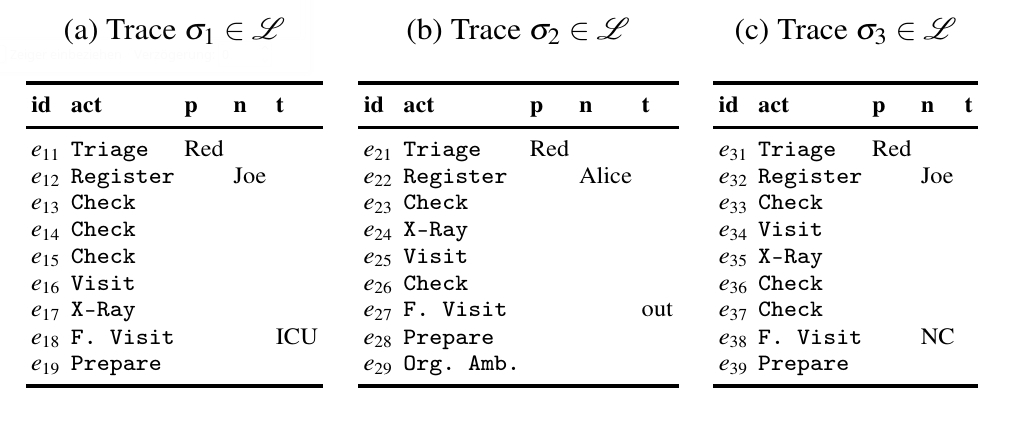
\includegraphics[width=14cm]{Chapters/Graphics_Paper/Event_Traces_ex_HB.jpg}
\caption{Three traces of an example process of the emergency ward data \protect\cite{Mannhardt17}} 
\end{figure}

\noindent While the data is presented in event logs - consisting of traces, the model derived from it, can be displayed in  graphical form (i.e. Petri net, C-net, BPMN). Common patterns, which can be displayed by a Petri net are Sequences, Choice [e, f], Parallelism [b, c, d], and Loops.

\begin{figure}[H]
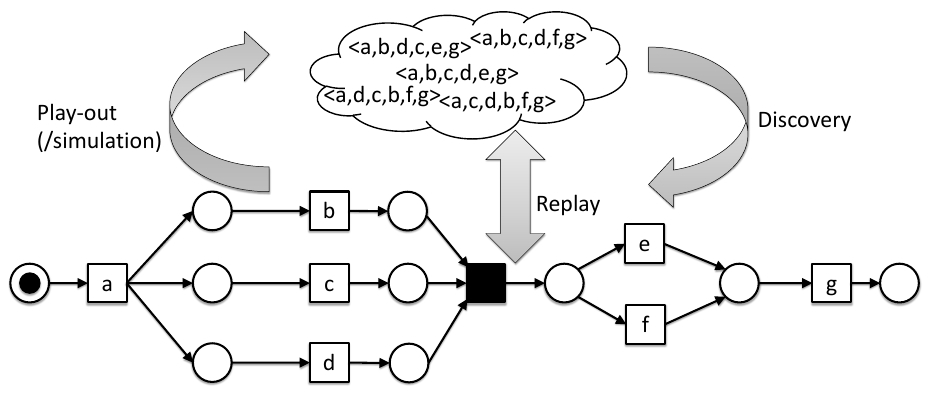
\includegraphics[width=14cm]{Chapters/Notizen_Graphics/ProcessModel_Behaviour.jpg}
\caption{A Petri net derived from Event logs\protect\cite{Buijs2017}} 
\end{figure}

\noindent Once a model has been discovered the following criteria should be considered:

\begin{enumerate}
\setlength{\itemsep}{3pt}
\item Soundness: Are the criteria for Soundness met?
\item Replay Fitness: Can all traces be represented by the model?
\item Precision: Can the model represent additional cases, not seen in the traces? 
\item Generalization: Is the model restrictive or can it be applied in general?
\item Simplicity: Is the model as simple as possible?
\end{enumerate}

\vspace{5mm}
\textbf{Soundness}
\begin{enumerate}
\setlength{\itemsep}{3pt}
\item{Option to complete}\\
For each possible state of the process model, it is possible to reach the end state

\item{Proper completion}\\
When the process model reaches the end state, there are no tokens left behind

\item{No dead transitions}\\
Each transition in the process model can be enabled\\
\protect\cite{Buijs2017}
\end{enumerate}



\subsection{Causal Nets}
Conventional model notations like Petri nets and BPMN are often not able to represent observed behavior properly and discovered process models tend to have dead- or livelocks. For this reason C-nets are preferred by the authors as representation for their DHM.\\
In a Causal-net (C-net) nodes represent activities and arcs represent causal dependencies. Each activity has a set of possible input bindings and a set of possible output bindings. For example in the following Figure the Activity "Register" has one input binding from "Triage" but two sets of output bindings \{"Check", "Visit"\}, \{"Check", "X-Ray"\}. This means that "Register" is either followed by "Check" and "Visit" or "Check" and "X-Ray".\protect\cite{Mannhardt17}\protect\cite{VanDerAlst11}

\begin{figure} [H]
    \subfigure{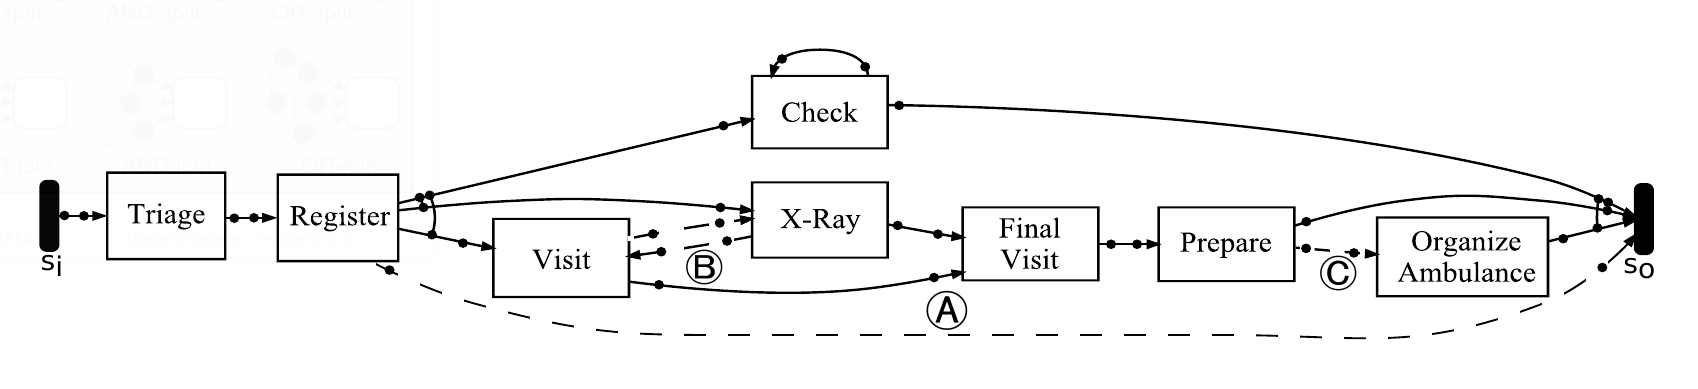
\includegraphics[width=0.7\textwidth]{Chapters/Graphics_Paper/C-net_ex_HB.jpg}}
    \subfigure{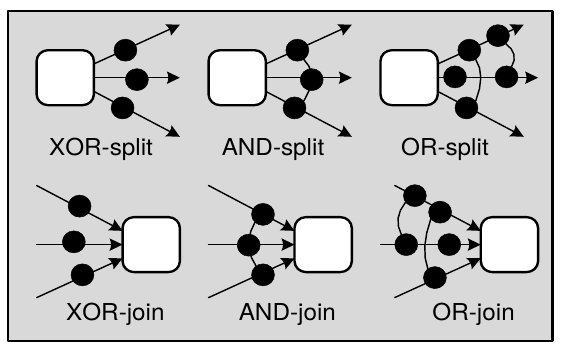
\includegraphics[width=0.25\textwidth]{Chapters/Graphics_Paper/C-nets_Legend.jpg}} 
\caption{Splits and Joins in a C-net of the emergency ward example process\protect\cite{Mannhardt17}\protect\cite{VanDerAlst11}} 
\end{figure}
\vspace{3pt}

\noindent In mathematical notation a C-net is a tuple $C = (\Sigma, s_i , s_o , D, I, O)$ , consisting of:
\begin{itemize}
\setlength{\itemsep}{2pt}
\item{$\Sigma$ finite set of activities}
\item{$s_i \in \Sigma$ unique start activity}
\item{$s_o \in \Sigma$ unique end activity}
\item{$D \subseteq \Sigma \times \Sigma$ dependency relation}
\item{$B = \{X \subseteq \mathscr{P} (\Sigma) \; \rvert \; X = \{ \varnothing \} \vee \varnothing \notin X \} $ possible bindings}
\item{$I \in \Sigma \rightarrow B$ set of input bindings per activity}
\item{$O \in \Sigma \rightarrow B$ set of output bindings per activity}\\
\protect\cite{Mannhardt17}
\end{itemize}



%----------------------------------------------------------------------------------------

\section{Mining Methods}
In order to discover an adequate process model the DHM builds on methods, which are applied in several established miners. The concepts of relation notation, footprint-/ dependency matrices and classification by decision trees in an event log, will be briefly introduced in connection to the respective miner.  

\subsection{Alpha Miner}
This very basic miner was the first to bridge from Event Logs to Petri nets. First a footprint matrix is detected from the event log. By applying the following notation, it can be interpreted from the symmetric matrix, that b follows a, but e, f and g never follow a.\\

\begin{tabular}[width=13cm]{llll}
$>$ & Directly follows &a $>$ b& a is directly followed by $b$ \\
$\rightarrow$ & Sequence & a $\rightarrow$ b & if $a>b$ and not $b>a$ \\
|| & Parallel & a || b & if both a > b and b > a \\
$\#$ & No direct relation & a $\#$ b & if neither $a>b$ and $b>a$ \\
\end{tabular}


\begin{figure}[H]
\begin{center}
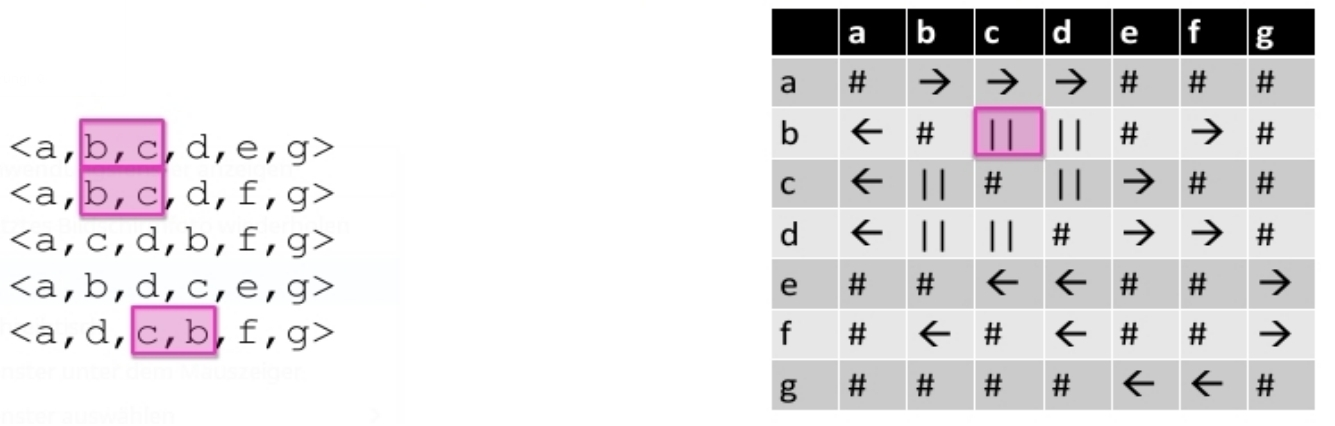
\includegraphics[width=0.8\textwidth]{Chapters/Graphics_Paper/AlphaMiner_DependenceMatrix.jpg}
\caption{The Footprint Matrix of the Alpha Miner\protect\cite{Buijs2017}} 
\end{center}
\end{figure}

\noindent From the footprint matrix the following Petri net can be derived. The actions b, c and d, which were marked as parallel in the above Figure, are now displayed as parallel paths.\protect\cite{Buijs2017}

\begin{figure}[H]
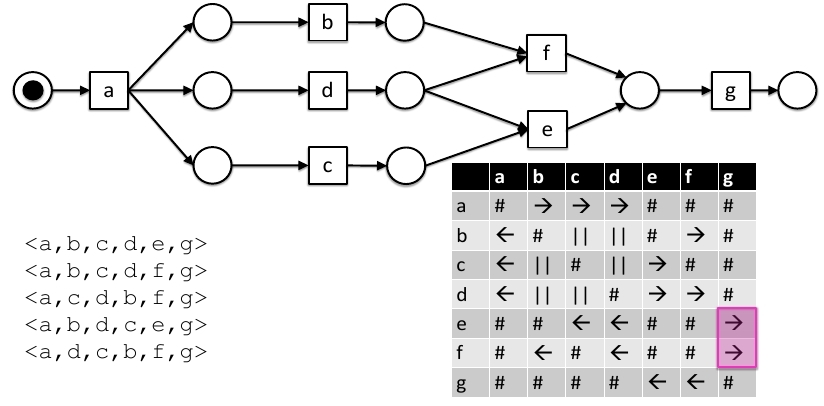
\includegraphics[width=0.9\textwidth]{Chapters/Notizen_Graphics/Notation_FootprintMatrix_PetriNet.jpg}
\caption{A derived Petri net of the Footprint Matrix\protect\cite{Buijs2017}} 
\end{figure}

\subsection{Heuristics Miner (HM)}
The Heuristic Miner is an Improvement of the Alpha miner, as it takes frequencies into account, detects short-loops and can detect skipping activities. However it does not guarantee for sound process models.\\

\noindent The basic idea is, to count the relations in the footprint matrix and calculate relative frequencies which returns a dependency matrix, as depicted in the following Figure.

\begin{figure}[H]
\begin{center}
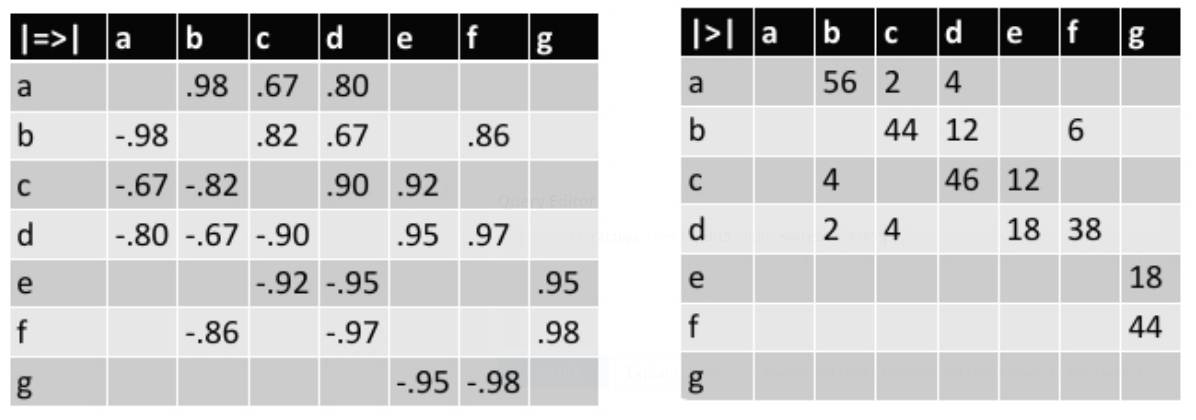
\includegraphics[width=0.7\textwidth]{Chapters/Graphics_Paper/HeuristicMiner_DependencyMatrix.jpg}
\caption{Dependency Matrix des Heuristic Miners\protect\cite{Buijs2017}} 
\end{center}
\end{figure}
\[a => b = \frac{|a>b|-|b>a|}{|a>b|-|b>a|+1}\]
\vspace{5pt}


\noindent It can be seen that the frequency of |a>b| - meaning a was followed by b - is 56. The opposite |b>a| never occurred and for this reason, by applying the formula above, the relative frequency or "significance of the dependency" of 0.98 can be calculated. The opposing relative frequency of -0.98 can be derived from the first result and is inserted in the matrix as well.\protect\cite{Buijs2017}


\subsection{Inductive Miner (IM)}
With the Inductive Miner the idea of classification by decision trees is introduced to process mining and because it doesn't use Petri nets, it guarantees sound process models.
The IM repeatedly finds the most prominent splits in the event log, then detects the operator (e.g. X) and afterwards continues on both sublogs.\\
In the following Figure the example event log from this chapter is first split into the most prominent activities a (start) and g (end). Afterwards the OR operator is applied for e and f and finally b,c and d are split with and the parallel operator detected for this split.\protect\cite{Buijs2017}

\begin{figure} [H]
    \subfigure[Always a]{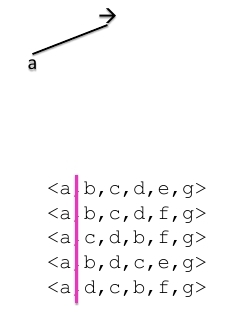
\includegraphics[width=0.34\textwidth]{Chapters/Notizen_Graphics/InductMin_repeat1.jpg}} 
    \subfigure[Always e OR f]{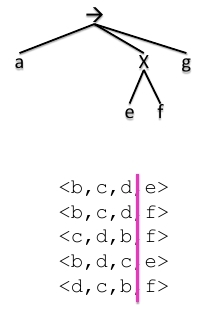
\includegraphics[width=0.3\textwidth]{Chapters/Notizen_Graphics/InductMin_repeat2.jpg}}
    \subfigure[Parallelism b,c,d]{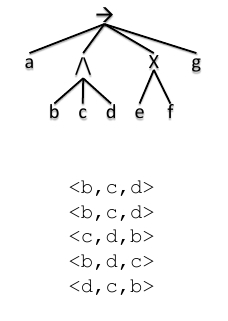
\includegraphics[width=0.33\textwidth]{Chapters/Notizen_Graphics/InductMin_repeat3.jpg}} 
\caption{Inductive Miner - Repeatedly Split Event Log\protect\cite{Buijs2017}} 
\end{figure} 


%----------------------------------------------------------------------------------------
\section{The Data-aware Heuristic Miner (DHM)}
\subsection{Data-aware Dependency Measures}
In contrast to the miners which have been shortly presented in this chapter, the DHM is supposed to also consider and evaluate infrequent but data-dependent process behavior. Rare events are either vastly disregarded as noise e.g. by the HM or not properly filtered e.g. by the IM.
\begin{figure} [H]
    \subfigure[Inductive Miner]{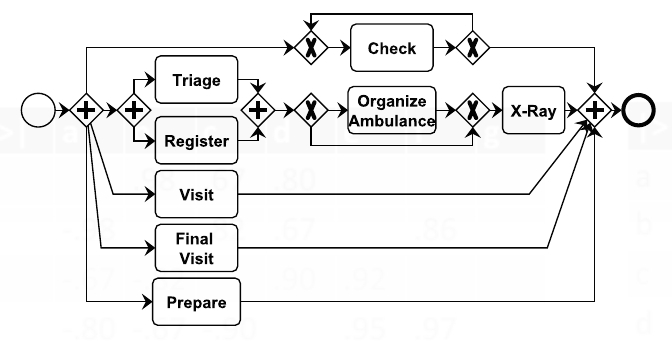
\includegraphics[width=0.49\textwidth]{Chapters/Graphics_Paper/IM_ex_HB.jpg}}
    \subfigure[Heuristic Miner]{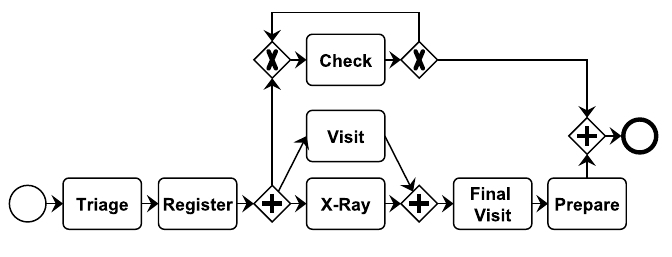
\includegraphics[width=0.49\textwidth]{Chapters/Graphics_Paper/HM_ex_HB.jpg}} 
\caption{Discovered models by the IM and HM in BPMN \protect\cite{Mannhardt17}}
\end{figure}

\noindent The approach of Mannhardt et. al is to extend the HM with a measure for conditional dependency. Binary classifiers are applied to predict directly-follows relations based on attribute values recorded in the event log.\\ 
\noindent Those classifiers are denoted as \textbf{Dependency Conditions}:
\[C_a,_b(x) = (C(a, b))(x)\]
This binary classifier predicts whether an event of activity a is directly followed by an event of activity b for the attribute values x. This means that $C_a,_b(x) = 1$ when b is predicted to directly follow a and $C_a,_b(x) = 0$ when a different activity is predicted.\\


\noindent Given $a, b \in \Sigma$ and dependency conditions C, the frequency with which b is observed to directly follow a is derived from the event log. This relation is denoted as:
\noindent\textbf{Conditional directly follows relation}
\[a >^{C,L} b\]
An execution of activity a with the latest attribute values x is directly followed by an execution of activity b under dependency condition $C_a,_b(x)$.

\noindent The \textbf{Conditional dependency measure} is calculated analogous to the dependency measure described for the HM earlier. The authors define 
$a => ^{C,L}b: \Sigma \times \Sigma \rightarrow [-1, 1]$ as the strength of the causal
dependency from a to b under condition $C_{a,b}$ in the event log:

\[a => ^{C,L}b = 
\begin{cases}
		\frac{|a>^{C,L}b|-|b>^{C,L}a|}{|a>^{C,L}b|-|b>^{C,L}a|+1} & \text{for a} \neq b,\\
		\frac{|a>^{C,L}b|}{|a>^{C,L}b|+1} & \text{otherwise}.
\end{cases}
\]

\noindent The difference to the earlier measure is the data-aware dependency condition. 
If a relation (a, b) is clearly characterized by a certain dependency condition $C_{a,b}$ it should be included in the dependency relations of the discovered causal net.\\

\noindent The \textbf{emergency ward example} will provide a better understanding of the described measures. An event log L with 50 traces for each of the three $\sigma_{1-3}$ was introduced earlier and will be used in the following steps:
\begin{enumerate}\setlength{\itemsep}{1pt}
\item Determine the conditional dependency measure $X => ^{C,L} V$ from activity X-Ray (X) to activity Visit (V)\\
=> Assumtion that condition $C_{X,V}(v) = 1$ only if attribute Nurse = Alice
\item Obtain the number of times X is directly followed by V under condition $C_{X,V}$\\
=> $|X >^{C,L} V|$ = 50
\item Obtain the number of times V is directly followed by X under conditions C \\
=> $|V >^{C,L} X|$ = 0
\item Derive the conditional dependency measure under C \\
=> $X => ^{C,L} V = \frac{50-0}{50+0+1} \approx 0.98$
\end{enumerate}
This indicates a strong dependency relation from activity X to activity V under condition $C_{X,V}$ . By contrast, if we consider the unconditional dependency measure $X => ^{1,L} V$, then we obtain $\frac{50-100}{50+100+1} \approx -0.33$.
Thus, when disregarding the data perspective, both activities appear to be executed in parallel.\protect\cite{Mannhardt17}

\subsection{Training a classifier for the dependency condition}
The \textbf{dependency condition} which was introduced above, is the basis of the other two definitions and thus the first step when applying the DHM in order to decide which relations should be included in the C-net.\\
A set of training instances is built for every combination of activities $(a, b) \in \Sigma \times \Sigma$.

\noindent \textbf{Training Instances} are defined by:
\begin{itemize}
\item $ a \in \Sigma$ the given source activity
\item $ b \in \Sigma$ the candidate activity
\item $ \theta_{dep} \in [0,1]$ the dependency threshold
\end{itemize}

\noindent Then $ a\bullet \subseteq \Sigma$ is the set of activities s that directly follow a in the event log with an unconditional dependency measure above the threshold $ \theta_{dep} $ , i.e., 
\[a\bullet = {s \in \Sigma | a => ^{1,L} s \geq \theta_{dep}}\]

\noindent We collect those events $X_{L,a,b} \subseteq E$ that directly follow an execution of a in the event log, and refer to activities in $a\bullet$, or to the candidate activity b, i.e.,  \[X_{L,a,b} = {e \in E | \bullet(e) = a \wedge \#_{act} (e) \in a\bullet \cup \{b\}}\]

\noindent Function $T_{L,\theta_{dep}}\in (\Sigma \times \Sigma) \rightarrow B((A \nrightarrow U) \times {1, 0})$ returns the multi-set of training instances:
\[T_{L,\theta_{dep}} (a, b) = \biguplus _{e \in X_{L,a,b}} [(val(e), cl(e))] with cl(e) =
\begin{cases}
1, & for \#_{act}(e)=b,\\
0, & for \#_{act}(e)\neq b
\end{cases}
\]

\noindent This method is conceptually independent of the used classification algorithm. The authors employed \textbf{decision trees (C4.5)} as they are efficient and provide results in human interpretable conditions.\\
To build the \textbf{dependency conditions C}:
\begin{enumerate}
\item A set of training instances $T_{L,\theta_{dep}} (a, b)$ is assembled.
\item A decision tree for each possible relation $(a, b) \in \Sigma \times \Sigma$ is trained.
\item A score $q(C_{a,b}) \in [0, 1]$ is used to determine the quality of a condition $C_{a,b}$.
\end{enumerate}

\noindent As a performance measure the authors opted for Cohen’s kappa ($\kappa$), which indicates whether the prediction was better than a prediction by chance (i.e., for $\kappa$ > 0).\\

\noindent Again the \textbf{emergency ward example} with an event log of 150 traces will provide a better understanding of the just described methods.\\
\noindent The dependency threshold shall be $\theta_{dep} = 0.9$ and the classifier for the dependency condition $C_{X,V}$, i.e., the dependency relation from X-Ray (X) to Visit (V) will be trained:

\begin{enumerate}
\item The training instances are $T_{L,\theta_{dep}}(X,V ) = [(v1, Final Visit)^{50} , (v2, Visit)^{50} ]$
\item The attribute value functions are $v1 (P) = Red$, $v1 (N) = Joe$ and $v2(P) = Red$, $v2 (N) = Alice$ 
\item A C4.5 decision tree is trained and the dependency condition $C_{X,V}$ with $C_{X,V} (v2 ) = 1$ and $C_{X,V} (v1) = 0$ is obtained
\end{enumerate}

\noindent There is no instance with the activity Check (C) since the unconditional dependency measure $X => ^{1,L}C$ is below the threshold of 0.9. So the instances based on trace $\sigma 3$ are not included because activity C is in parallel to X.\protect\cite{Mannhardt17} 

\subsection{Tuning noise filtering capabilities and discovering C-nets}
In order to filter the noise from rare events the DHM supports four user-specified thresholds which range between 0 and 1:
\begin{itemize}
\item $\theta_{obs}$, observation threshold - controlling the relative frequency of relations
\item $\theta_{dep}$, dependency threshold - controlling the strength of causal dependencies
\item $\theta_{bin}$, binding threshold - controlling the number of bindings
\item $\theta_{con}$, condition threshold - controlling the quality of data dependencies
\end{itemize}

\noindent A C-net tuple $C = (\Sigma, s_i , s_o , D, I, O)$ is derived from an event log $L = (E, \Sigma, \#, L)$ and the thresholds $\theta_{obs}$, $\theta_{dep}$, $\theta_{bin}$, $\theta_{con}$, in the following steps.

\begin{enumerate}
\item Add artificial start and end events to all traces to ensure unique start and end activities $s_i$ and $s_0$
\item Build the set of standard dependency relations
\item Discover the dependency conditions C by training the classifiers for each pair (a, b), using the training instances $T_{L,\theta_{dep}} (a, b)$.
\item Add the conditional dependency relations C to D, using $\theta_{con}$ instead of $\theta_{obs}$ to
obtain infrequent, high-quality data conditions
\item Handle activities $s \in \Sigma$ which don't have a predecessor or successor in the directed
graph induced by D. As all tasks in the C-net should be connected, two alternative heuristics are proposed by the authors: \textbf{all-task-connected} and \textbf{accepted-task-connected}. The latter one connects repeatedly only those activities that are already part of the dependency graph using their best neighboring activities until all activities have a cause and an effect.\\
$\bar{D}$ denotes the set of relations necessary to connect all activities accepted so far. Afterwards the dependency relations with the new relations, i.e., $D = D \cup \bar{D}$ is extended. As now there might be new, unconnected activities in $\bar{D}$ the steps are repeated i.e. the best neighboring activities are added until set $\bar{D}$ is empty.
\item The input and output binding functions of the C-net are discovered. We discover the input ($I$) and output ($O$) binding functions of the C-net. To find $O(a)$ it has to be determined which of the executions of b were caused by an execution of activity a. Using the same heuristic like before activity a only is considered to have caused b if it is the nearest activity. Any other activity s executed in between a and b should not be a possible cause of b. $\bar{O}$ denotes the set of activities that were caused by event $e_i$.

The frequency $|o|_{L,a} \in N$ of an output binding $o \subseteq \Sigma$ for activity $a \in \Sigma$
in the event log L is determined as:
\[O(a) = \{{o \subseteq \Sigma | \frac{|o|_{L,a}}{max_{\bar{o}\subseteq \Sigma}(|\bar{o}|_{L,a})}\geq \theta_{bin}}\}\]\\
The input binding function $I$ is obtained by reversing the same approach.\protect\cite{Mannhardt17}
\end{enumerate}


























